\chapter{Sviluppo software}
\label{cap:sviluppo-software}

\section{Design dei Sistemi}
Nell'ambito dello sviluppo software ho implementato quello che si chiama \textit{Design di Sistemi}.\\
Il Design dei Sistemi (Systems Design) è stato essenziale per comprendere e gestire le interazioni tra le varie componenti del sistema. Questo approccio mi ha permesso di assicurare che tutte le parti dell'interfaccia lavorassero insieme in modo coerente ed efficiente.\\
Ho analizzato l'architettura del sistema, identificando tutte le componenti principali e le loro interazioni. Questo includeva il backend, il frontend, e le API utilizzate per la comunicazione tra le diverse parti del sistema.\\
L'obiettivo era garantire che il frontend fosse perfettamente allineato con le funzionalità offerte dal backend, facendo da filtro iniziale per prevenire l'errore nell'utente ed evitare il rischio di atterrare in pagine di errore di difficile gestione o comprensione per l'utente inesperto. \\

Per implementare il Design dei Sistemi, ho utilizzato un approccio modulare, suddividendo l'interfaccia in componenti riutilizzabili. Ogni componente è stato progettato per essere indipendente e facilmente integrabile con gli altri, seguendo i principi della progettazione a strati.\\
Ho separato il frontend (React) dal backend (Flask), garantendo che ciascuno potesse essere sviluppato, testato e aggiornato indipendentemente. Questa separazione ha facilitato non solo la manutenzione del software, ma anche l'implementazione di nuove funzionalità, permettendo un'evoluzione più rapida del prodotto.\\


\section{Il progetto in partenza}
Il software nasceva come POC, era un monolite unico dove backend e frontend risiedevano nella stessa directory.\\
Il backend, scritto in python, si occupava di:
\begin{itemize}
    \item esporre un endpoint per il frontend 
    \item realizzare calcoli di machine learning per generare le visualizzazioni 
\end{itemize}

Il frontend invece era composto da tre due file html, uno per il form e uno per la visualizzazione dei grafici, due file javascript, uno per la validazione del form e uno per la realizzazione dei grafici, e un file css che dava lo stile a tutto. 

\section{Analisi e motivazioni}

Dopo una prima analisi del software ho proposto di operare una divisione più netta di frontend e backend avvalendomi dell'ausilio di un framework per il frontend. Attraverso questa scelta si è seguito il principio di progettazione architetturale noto come \textit{Architettura a Strati} o \textit{Architettura a Livelli} (Layered Architecture).

Nell'architettura a strati, l'applicazione è suddivisa in diversi strati logici o livelli, ognuno dei quali ha una responsabilità specifica. Nel mio caso:
\begin{enumerate}
\item Backend (Strato logico):
    \begin{itemize}
        \item  Responsabilità: Gestisce la logica di presentazione, in particolare la generazione delle risposte API per il frontend.
        \item  Tecnologie utilizzate: Flask, Python, API REST.
    \end{itemize}
\item Frontend (Strato di Presentazione):
 \begin{itemize}
    \item Responsabilità: Interagisce con l'utente e invia richieste API al backend per ottenere e visualizzare i dati.
    \item Tecnologie utilizzate: React, JavaScript, HTML, CSS.
    \end{itemize}
\end{enumerate}

Questa separazione ha permesso di ottenere la divisione delle responsabilità, facilitando la manutenzione e l'aggiornamento dei singoli componenti senza influenzare gli altri.\\
La modularità introdotta permette inoltre di scalare l'applicazione con maggiore facilità, ad esempio nel caso in futuro si volesse applicare moduli di registrazione e login, quindi avere cura della sicurezza, oppure ampliare il numero di grafici da mostrare all'utente. \\
Il mio focus era principalmente la possibilità di ampliare il software operando un limitato numero di modifiche, quindi portare il frontend e la gestione dei grafici ad una discreta maturità.

\section{Sviluppi}
Gli sviluppi sono proseguiti in parallelo tra me e i colleghi che ho assistito. Io mi sono occupata principalmente del frontend, sono partita dall'interfaccia del wizard mentre ho assistito i colleghi nella realizzazione di endpoint e sistemazione del backend.\\
Dapprima sono stati realizzati endpoint separati per la validazione e il submit del form relativo ai dati del paziente. Successivamente, su mia sollecitazione, le logiche sono state accorpate in un unico endpoint che rispondesse con la visualizzazione oppure elencasse i campi non validi. La validazione è stata implementata sia lato frontend che lato backend per garantire maggiore robustezza.\\

\subsection{React}
Il frontend è stato sviluppato in React, le principali librerie usate sono state:
\begin{itemize}
    \item \textbf{Bootstrap}: Per lo stile e alcuni componenti preconfezionati.
    \item \textbf{Axios}: Per le chiamate API.
    \item \textbf{Toastify}: Per mostrare notifiche (toast) in fase di validazione del form del paziente.
\end{itemize}

Queste librerie sono state installate attraverso il package manager npm, facilitando la gestione delle dipendenze del progetto. Il vantaggio di npm è l'accesso a migliaia di pacchetti open source, rendendo più semplice l'aggiornamento e la gestione delle librerie utilizzate, e la messa a disposizione di script di build per effettuare il build e deploy del progetto. 

\subsection{Flask}
Flask è un microframework per Python, è stato scelto per la sua semplicità e flessibilità in quanto consente di costruire applicazioni web leggere e modulari.
Nel mio caso ho operato modifiche anche al backend, in particolare nella risposta inviata al frontend per calcolare le visualizzazioni. In origine, tra i campi modificabili vi era l'età, ma a seguito di analisi si è concluso che non era una dimensione di interesse per il medico-utente. Pertanto è stata sostituita con il peso.\\ 
Ho inoltre predisposto la POST degli endpoint che ricevono i form di valutazione dell'utente, in modo tale che il collega maggiormente incentrato sul backend potesse successivamente sviluppare le feature per il salvataggio a CSV del form compilato.\\
La struttura del backend è così composta: 
\begin{itemize}
    \item \textbf{flaskapp.py}: è il punto d'ingresso principale per lanciare il progetto e contiene le rotte e le logiche di gestione delle richieste.
    \item \textbf{utils.py}: è il file dove sono presenti tutte le funzioni che si occupano di realizzare le visualizzazioni da inviare al frontend.
\end{itemize}

\subsection{Validazione}
Il software opera una doppia validazione:
\begin{itemize} 
    \item una lato frontend quando l'utente compila i campi, in modo tale da avere subito feedback se qualcosa non è corretto; questa viene fatta tramite chiamata a funzioni di validazioni implementate inizialmente dalla collega e successivamente evolute da me affinchè funzionassero in ambiente React. 
    \item una lato backend, il quale controlla il form pervenuto e verifica se sia tutto conforme.\\
\end{itemize}

Se lato frontend non dovessero esserci segnalazioni di errori, ma al contrario il backend dovesse rispondere con un errore, questo viene notificato al frontend e l'utente può vedere a video una pagina di errore con la descrizione di cosa è andato storto. Nel caso in cui il backend dovesse rispondere errore 500 l'utente vedrà una pagina di errore con descrizione generica. 

\subsection{La struttura}
Le pagine principali sono le seguenti:\\ 
\begin{itemize}
    \item \textbf{Wizard:} è presente il wizard iniziale dove l'utente compila i dati del paziente; si compone di 2 step:  il primo è la scelta della zona da operare, il secondo è l'effettivo inserimento manuale dei dati del paziente.
    \item \textbf{Results:} è la pagina di risultati dove l'utente visualizza i grafici e interagisce con gli stessi.
    \item \textbf{Evaluation:} è la pagina di valutazione dell'applicativo, dove è presente un form che l'utente può compilare per darci il suo feedback. 
    \item \textbf{Tutorial:} è una pagina accessibile dall' header che descrive l'applicativo e funge appunto da tutorial per l'utente. 
\end{itemize}
All'interno di queste pagine è possibile trovare diversi componenti necessari a suddividere ulteriormente la complessità delle pagine e delle logiche.\\ 
Abbiamo quindi il componente per l'header, gli step del wizard, il contenuto della dialog.\\

Nota importante è l'utilizzo del \textit{global context}, ovvero un contesto globale che permette di condividere informazioni tra i diversi componenti senza dover sottostare alla relazione parent-child. All'interno del global context possiamo trovare la gestione degli step, gran parte del formi iziale compilato dall'utente in quanto molte informazioni sono necessarie in più pagine e componenti, i dati fetchati in quanto servono alla pagina Results per calcolare le visualizzazioni. Il global context si occupa anche di controllare anche se parte di questi dati sono già presenti nel local storage del browser, quindi di inizializzare le rispettive strutture dati.\\

La costruzione del wizard compilato dall'utente avviene in maniera dinamica, questo vuol che in base alla prima preferenza espressa dall'utente (spine o hip/knee) i campi da compilare cambieranno. Questa scelta è stata implementata per più motivi: il primo è che inizialmente le operazioni da esplorare erano tre, ovvero hip, knee, spine; il secondo è che in base alla scelta dell'utente i campi del form erano effettivamente diversi, ed era ridondante utilizzare componenti react differenti in base al form necessario. Per implementare questa feature mi sono avvalsa dell'uso di un JSON di dati, dove viene inserita la lista di campi che devono comparire e le loro caratteristiche, ovvero con che nome devono essere inviati a backend, che tipo sono (number, text, select, radio) e quale sarà la funzione che si occuperà dalla validazione; il terzo è che qualora si volessero ampliare le parti del corpo operate che un medico può esplorare basterà aggiungere il corrispettivo delle voci a backend anche a frontend, limitanto quindi le modifiche da apportare ad due soli file per il frontend (il JSON con la lista dei campi e la lista di funzioni di validazione). 

\begin{figure}[!ht] 
    \centering 
    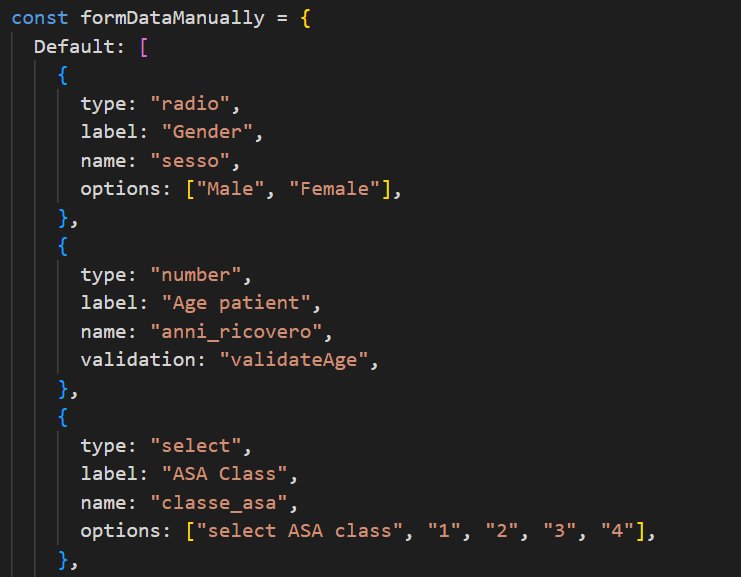
\includegraphics[width=0.9\columnwidth]{dynamic-form-example} 
    \caption{Natura dell'incertezza}
\end{figure}

